
\section{Elección de perfil}

En esta sección se elige el perfil aerodinámico que montará el ala. Son necesarios cuatro requisitos en este: número de Reynolds $\left( \reynolds \right)$ mínimo adecuado, espesor relativo $\left( t/c \right)$ mayor al $10\%$, eficiencia aerodinámica $\left( E = L / D \right)$ elevada y momento libre $\left( C_{m0} \right)$ ligeramente positivo. 

Según \cite{performace_hoIV}, las cuerdas de raíz y de punta del Ho IV son $c_r = 1.55 \ \meter$ y $c_t = 0.28 \ \meter$. Se asume una velocidad de vuelo de $100 \ \kilo\meter / \hour$ y atmósfera ISA a nivel del mar, $\rho = 1.225 \ \kilo\gram$ y $\mu = 1.789 \cdot 10^{-5} \ \pascal \cdot \second$. Tomando las cuerdas raíz y de punta como longitudes características, los Reynolds en las secciones son $\reynolds_r = 2.95 \cdot 10^6$ y $\reynolds_t = 5.30 \cdot 10^5$.

La referencia \cite{aerotools_1} propone una serie de perfiles con los requisitos adecuados para alas volantes. Estos se recogen en la tabla \ref{tab:posibles_perfiles}.
\begin{table}[h]
    \centering
    \begin{tabular}{llll}
        \toprule[0.50mm]
        Perfil & $t/c \ \left( \% \right)$ & $C_{m0}$ & $\reynolds_\text{min}$ \\
        \midrule[0.25mm]
        MH 60   & $10.12$ & $0.0140$ & $150 \kilo$ \\
        MH 61   & $10.28$ & $0.0175$ & $150 \kilo$ \\
        MH 91   & $14.47$ & $0.0326$ & $-$ \\
        MH 92   & $19.96$ & $0.0374$ & $-$ \\
        MH 104  & $15.30$ & $0.0090$ & $500 \kilo$ \\
        MH 106  & $13.00$ & $0.0200$ & $500 \kilo$ \\
        MH 108  & $12.00$ & $0.0220$ & $500 \kilo$ \\
        MH 110  & $10.00$ & $0.0410$ & $500 \kilo$ \\
        \bottomrule[0.50mm]
    \end{tabular}
    \caption{Perfiles aerodinámicos con espesor relativo $\left( t/c \right)$, momento libre $\left( C_{m0} \right)$ y número de Reynolds mínimo $\left( \mathrm{Re}_\text{min} \right)$ adecuados para el Ho IV. A partir de \cite{aerotools_1}.}
    \label{tab:posibles_perfiles}
    \vspace{-4mm}
\end{table}

\noindent
El $\reynolds_\text{min}$ de los perfiles $\mathrm{MH}\,104$ a $\mathrm{MH}\,110$ es cercano a $\reynolds_t$. En condiciones de vuelo con menor densidad, \eg, a mayor altura de vuelo, puede darse $\reynolds < 5 \cdot 10^5$. Por debajo de $\reynolds_\text{min}$ el comportamiento de la capa límite tiene gran influencia sobre el rendimiento del perfil, pudiendo desprenderse antes de lo esperado. Esto supone un riesgo para la operación segura de la aeronave. Por consiguiente, únicamente son adecuados los perfiles $\mathrm{MH}\,60$ y $\mathrm{MH}\,61$.

Ambos perfiles tienen un espesor relativo ligeramente superior al $10\%$. Esto permite trabajar la distribución de presión modificando más ampliamente la curvatura del intradós y extradós. A su vez, se obtiene un $C_{m0}$ positivo, en el rango $0.010$ -- $0.020$, el cual es adecuado para el ala volante, pues contribuye a su estabilidad longitudinal.

El último criterio para la elección de los perfiles es la eficiencia aerodinámica. A partir de los datos experimentales proporcionados en \cite{aerotools_1} se pueden representar las curvas de eficiencia aerodinámica, mostradas en la figura \ref{fig:mh60_mh61_efficiency}. Los $\reynolds$ elegidos son los más cercanos a $\reynolds_r$ y $\reynolds_t$. Se aprecia que, en general, el perfil $\mathrm{MH}\,60$ tiene mayor $E$ para todo $\alpha$ y $\reynolds$. Se considera por lo tanto que este es el perfil adecuado para el Ho IV.
\begin{figure}[ht]
    \centering
    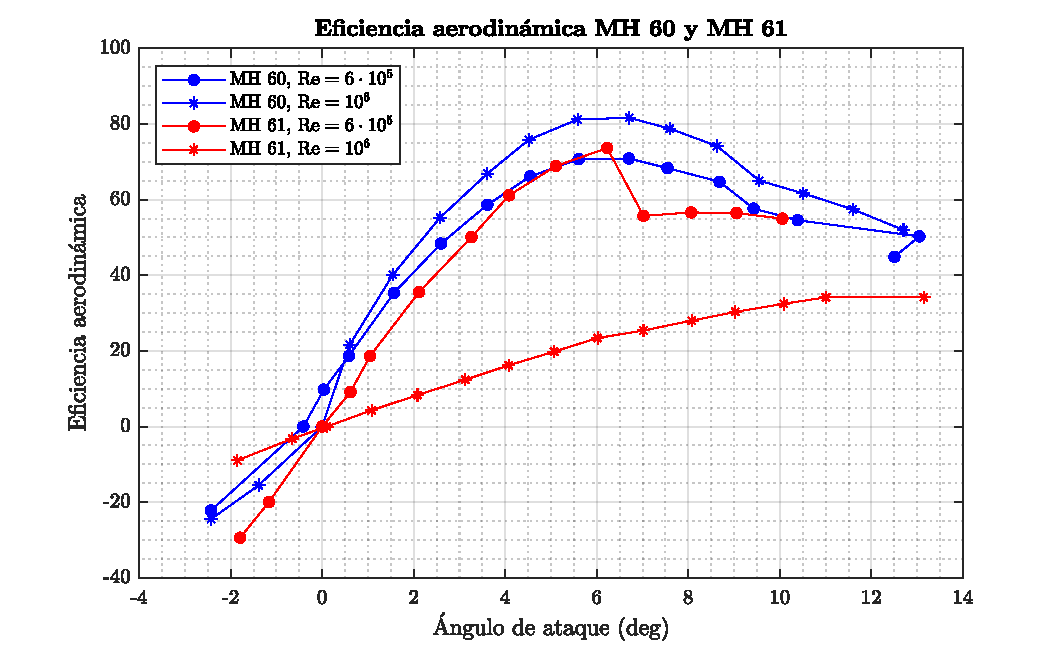
\includegraphics[width=\linewidth]{imagenes/eleccion_perfil/mh60_mh61_efficiency.pdf}
    \caption{Eficiencia aerodinámica $\left( E \right)$ en función del ángulo de ataque $\left( \alpha \right)$ para los perfiles $\mathrm{MH}\,60$ y $\mathrm{MH}\,61$, en $\reynolds = 6 \cdot 10^5$ y $\reynolds = 10^6$.}
    \label{fig:mh60_mh61_efficiency}
    \vspace{-4mm}
\end{figure}

Con los datos experimentales se calcula la regresión lineal de $C_l = f \left( \alpha \right)$ para obtener la pendiente de sustentación $\left( C_{l\alpha} \right)$ y el ángulo de sustentación nula $\left( \alpha_{l0} \right)$. Solamente se utilizan los puntos en el rango de $\alpha$ de $-2\degrees$ a $8\degrees$, \ie, en el régimen lineal. Del mismo modo se calcula la regresión lineal de la curva polar $C_d = f \left( C_l^2 \right)$ y se obtienen el coeficiente $k$ y la resistencia parásita $\left( C_{D0} \right)$. Para obtener buena aproximación de $C_{D0}$, los puntos para la regresión se sitúan en el rango de $C_l$ de $0$ a $0.8$. Los coeficientes obtenidos para ambos $\reynolds$ se recogen en la tabla \ref{tab:coeficientes_mh60}.
\begin{table}[ht]
    \centering
    \begin{tabular}{lllll}
        \toprule[0.50mm]
        $\reynolds$ & 
        $C_{l\alpha} \, \left( \deg^{-1} \right)$ & 
        $\alpha_{l0} \, \left( \deg \right)$ & 
        $C_{D0} \, \left( 10^{-3} \right)$ & 
        $k \, \left( 10^{-3} \right)$ \\
        \midrule[0.25mm]
        $600k$ & $0.1080$ & $-0.4355$ & $8.624$ & $5.853$ \\
        $1000k$ & $0.1095$ & $-0.3519$ & $7.174$ & $5.257$ \\
        \bottomrule[0.50mm]
    \end{tabular}
    \caption{Pendiente de sustentación $\left( C_{l\alpha} \right)$, ángulo de sustentación nula $\left( \alpha_{l0} \right)$, coeficiente de resistencia parásita $\left( C_{D0} \right)$ y coeficiente $k$ en $\reynolds = 6 \cdot 10^5$ y $\reynolds = 10^6$ para $\mathrm{MH}\,60$.}
    \label{tab:coeficientes_mh60}
    \vspace{-4mm}
\end{table}

En las figuras \ref{fig:mh60_lift} y \ref{fig:mh60_polar} se representan la curva de sustentación y la polar de resistencia para el $\mathrm{MH}\,60$. Se aprecia que las curvas de $C_l$ son muy similares para ambos $\reynolds$. A medida que $\reynolds$ crece, la capa límite es más energética y el desprendimiento se da más cerca del borde de salida. Por consiguiente, la resistencia de presión disminuye, como se refleja en la polar de resistencia. 
\begin{figure}[ht]
    \centering
    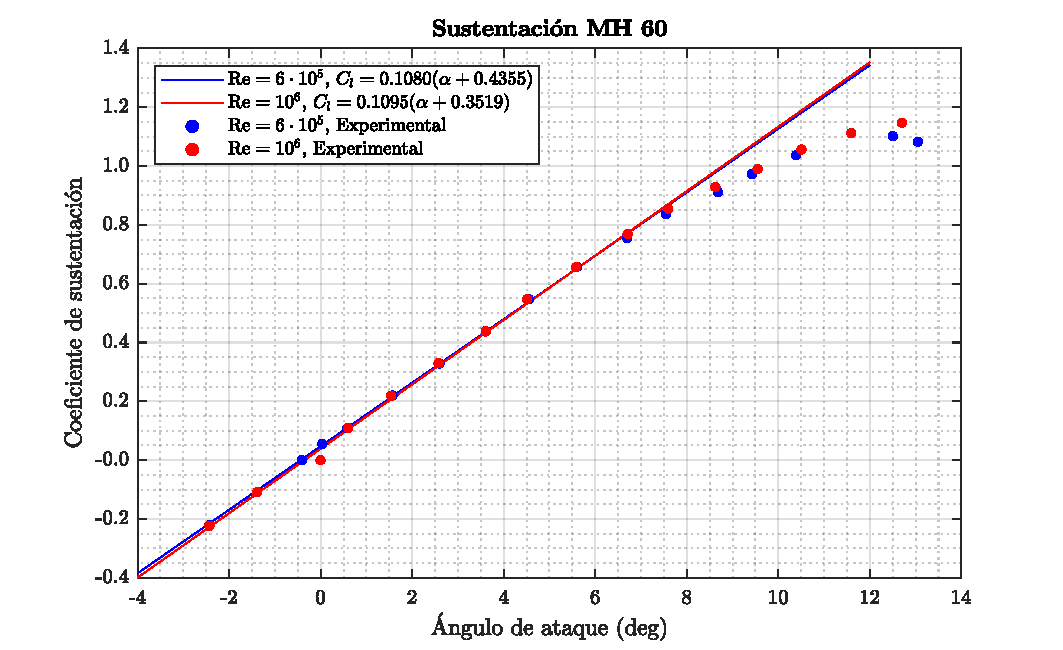
\includegraphics[width=\linewidth]{imagenes/eleccion_perfil/mh60_lift.pdf}
    \caption{Curva de sustentación $\left( C_l = f \left( \alpha \right) \right)$ del perfil $\mathrm{MH}\,60$ para $\reynolds = 6 \cdot 10^5$ y $\reynolds = 10^6$.}
    \label{fig:mh60_lift}
    \vspace{-4mm}
\end{figure}

\begin{figure}[ht]
    \centering
    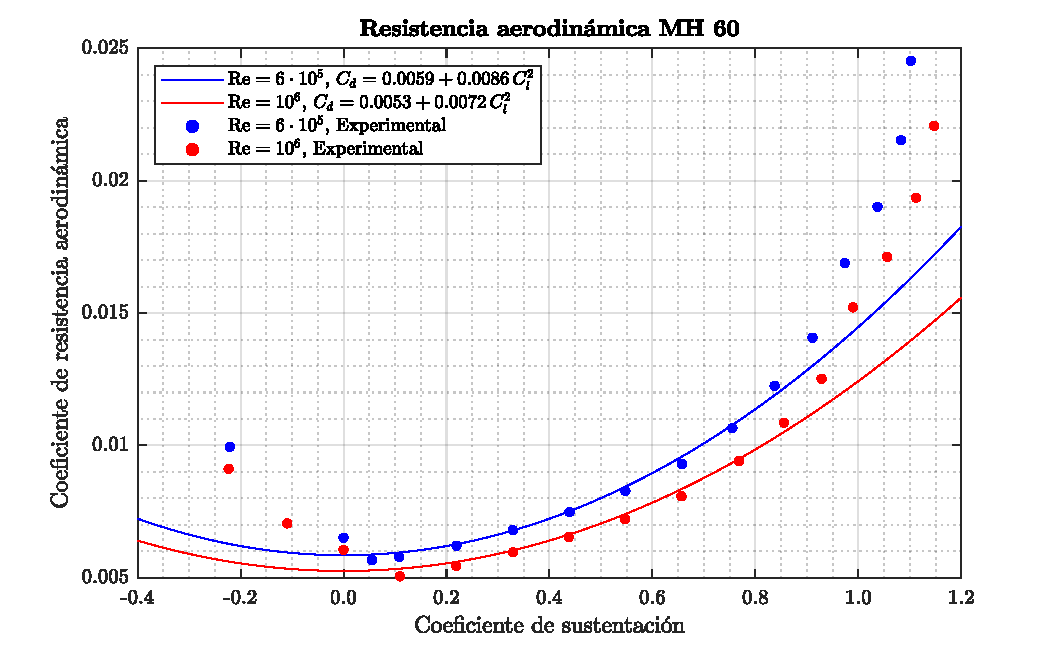
\includegraphics[width=\linewidth]{imagenes/eleccion_perfil/mh60_polar.pdf}
    \caption{Polar de resistencia $\left( C_d = f \left( {C_l}^2 \right) \right)$ del perfil $\mathrm{MH}\,60$ para $\reynolds = 6 \cdot 10^5$ y $\reynolds = 10^6$.}
    \label{fig:mh60_polar}
    \vspace{-4mm}
\end{figure}


